
\chapter{Usage}

\section{Main Modules}
\label{main_modules}

The core is split in three main modules:

\begin{enumerate}
    \item The CPU (mips\_cpu.vhdl).
    \item The cache+memory controller (mips\_cache.vhdl).
    \item An 'MCU' entity which combines CPU+Cache (mips\_mpu.vhdl).
\end{enumerate}

The entity you should use in your projects is the MCU module. The project 
includes a 'hardware demo' built around this module (see section 
~\ref{pregenerated_demo}) which can be used as an usage example.\\

The main modules are briefly described in the following subsections.


\section{MCU Module}
\label{mcu_module}

The MCU module main purpose is to encapsulate the somewhat complex 
interconnection between the CPU and the Cache module.

If some project demands that some piece of hardware be directly connected to the
CPU, bypassing the cache, this is where it should be -- an MMU comes to mind.

Any peripherals deemed common enough that they will be present in all projects
might be placed in the MCU module too -- after all, the MCU name has been chosen
to imply that 'bundling together' of a CPU and a bunch of peripherals.

In the current version of the MCU module, there is only a peripheral included in 
it -- a hardwired UART module. There is no penalty for placing peripherals 
ouside the MCU module, so there is no incentive to place them inside, thus 
making the interface more complex. This is an implementation option of yours.\\

\subsection{MCU Ports}
\label{mcu_ports}

\begin{figure}[h]
\makebox[\textwidth]{\framebox[9cm]{\rule{0pt}{9cm}
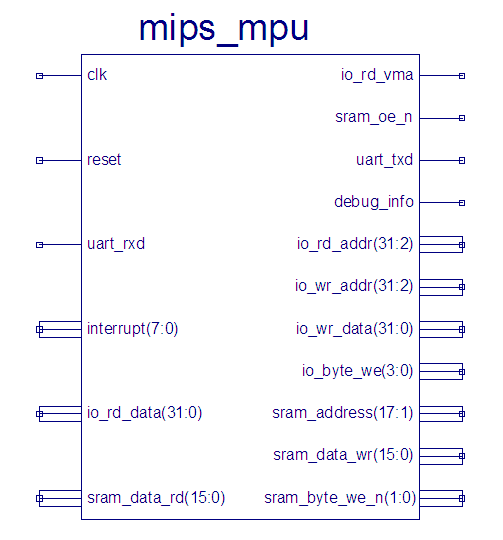
\includegraphics[width=8cm]{img/mpu_symbol.png}}}
\caption{MPU module interface\label{mpu_symbol}}
\end{figure}

\begin{table}[h]
\caption{MCU module interface ports}
\begin{tabularx}{\textwidth}{ lll|X }
\toprule
Name & Type & Width & Description \\
\midrule
clk                 & in    & 1  & Clock input, active rising edge. \\
reset               & in    & 1  & Synchronous global reset. \\
\midrule
sram\_address       & out   & 16 & Memory word address (bit 0 absent). \\
sram\_data\_wr      & out   & 16 & Memory write data. Only valid when one of the \\
                    &       &    & memory byte write enable outputs is active.\\
sram\_data\_rd      & in    & 16 & Memory read data. Latched when xxx. \\
sram\_byte\_we\_n   & out   & 2  & Memory byte write enable, active low.  \\
                    &       &    & (0) enables the low byte (7 downto 0) \\
                    &       &    & (1) enables the high byte (15 downto 8). \\
\midrule
io\_rd\_addr        & out   & 30 & I/O port read address (bits 1..0 absent). \\
                    &       &    & Only valid when io\_rd\_vma is high. \\
io\_wr\_addr        & out   & 30 & I/O port write address (bits 1..0 absent). \\
io\_wr\_data        & out   & 32 & I/O write data.  Only valid when one of the \\
                    &       &    & i/o byte write enable outputs is active.\\
io\_rd\_data        & in    & 32 & I/O read data. Latched when xxx. \\
io\_byte\_we        & out   & 4  & I/O byte write enable, active high. \\
                    &       &    & (0) enables the low byte (7 downto 0) \\
                    &       &    & (3) enables the high byte (31 downto 24). \\
io\_rd\_vma         & out   & 1  & Active high on i/o read cycles. \\
\midrule
uart\_rxd           & in    & 1  & RxD input to internal UART. \\
uart\_txd           & out   & 1  & TxD output from internal UART. \\
\midrule
interrupt           & in    & 8  & Interrupt request inputs, active high. \\
\bottomrule
\end{tabularx}
\end{table}

As you can see in figure~\ref{mpu_symbol} (symbol generated by Xilinx ISE), 
the MCU has the following interfaces:

\begin{enumerate}
    \item Interface to external static asynchronous memory (SRAM, FLASH...).
    \item Interface to on-chip peripherals.
    \item Interrupt inputs.
\end{enumerate}

These interfaces will be explained in the following subsections. The top module
for the demo supplied with the project (c2sb\_demo.vhdl) will be used for 
illustration.

\emph{NOTE}: This section needs a lot of elaboration -- ideally this should be 
equivalent to 
a datasheet in thoroughness and detail. This work, like many other parts of this
project, will have to wait.

\subsection{MCU interface to static memory}
\label{mcu_if_sram}

The interface to external memory in the MCU module is essentially that of the 
internal cache/memory controller. Its timing is described in section 
~\ref{cache_state_machine}.\\

The MCU inputs are meant to be connected straight to the FPGA i/o pins. The only
trick is the bidirectional memory data bus: as you can see, the MCU data buses 
are unidirectional and thus you will need to provide an interconnection
external to this module. This interconnection shall include the requisite 
3-state buffers:

\begin{verbatim}
sram_databus <= sram_data_wr when sram_byte_we_n/="11" else (others => 'Z');
\end{verbatim}

The top level module can be used as a fully tested example of how to use this 
interface to connect to a common SRAM chip (ISSI IS61LV25616).

In reviewing the top module source, note that I had to adapt the dual 
byte-write-enable outputs to the SRAM
configuration of a single write-enable plus dual byte-enable inputs.

Note too that the static memory bus is used to access both the 16-bit wide SRAM 
and an 8-bit wide FLASH. These chips are connected to separate buses on the 
target board, so the top module needs to conflate both buses before connecting 
them to the MPU. This is why a multiplexor is used in the mpu\_sram\_data\_rd
bus. A real-world board would probably have the SRAM and the FLASH connected 
to the same bus, simplifying the interface logic.
   
    
\subsection{MCU interface to peripherals}
\label{mcu_if_io}

    TODO Documentation to be done

\subsection{MCU interrupt inputs}
\label{mcu_irqs}

    TODO Documentation to be done
